\documentclass[12pt]{scrartcl}

\usepackage[american]{babel}

\usepackage{graphicx}
\graphicspath{{images/}}

\usepackage{paralist}
\usepackage{csquotes}
\usepackage[T1]{fontenc}
\usepackage{lmodern}
\usepackage[marginal]{footmisc}
\usepackage{hyperref}

\usepackage{geometry}
% \geometry{a4paper,body={5.8in,9in}}
\geometry{a4paper}

\usepackage{amsmath, amsfonts, amssymb}
\usepackage{placeins}
\usepackage{subcaption}

\usepackage{setspace}

\setlength{\parindent}{0pt}
%
%%%%%%%%%%%%%%%%%%%%%%%%%%%%%%%%%%%%%%
% ab hier steht der eigentliche Text:
\begin{document}

\title{Automatic Ranking of Classification Algorithms}
\subtitle{A Comparison of Regression-Based Ranking and Preference Models
\\\vspace{2em}Bachelor Thesis Proposal \& Work Plan}

\author{Helena Graf\\ 
\small{matriculation number: 7011643}\\ 
\small{hgraf@mail.upb.de}}
\date{\today}

\maketitle
\vspace{2em}

\begin{center}
\small{Supervisors:}\\
\large{Prof. Dr. Eyke H\"ullermeier}\\
\large{Prof. Dr. Axel-Cyrille Ngonga Ngomo}
\end{center}

\newpage
\tableofcontents
\newpage

\section{Motivation}\label{sec:motivation}
Selecting a fitting classifier for a new problem is difficult, since algorithm performances can vary substantially among datasets, and it is not feasible to simply apply a large number of them to empirically to find a good match. For example, on a dataset about the electricity prices in the Australian state New South Wales, %TODO cite
 the predictive accuracy for the Multilayer Perceptron\footnote{Hyperparameters: L:0.3,M:0.2,N:500,V:0,S:0,E:20,H:a.} is 0.7887 %TODO cite
. The predictive accuracy of the Random Forests\footnote{Hyperparameters: P:100,I:100,num-slots:1,K:0,M:1.0,V:0.001,S:1.} algorithm on the same data set is 0.9236, a much higher value. %TODO cite
On a different data set, with the topic of vehicle silhouetes, %TODO cite
 we get a predictive accuracy of 0.7979 %TODO cite
 for the Multilayer Perceptron, and 0.7518 %TODO cite
 for Random Forests, showing an advantage of the former on this dataset\footnote{Hyperparameters as above.}. So in each case, one would have picked a different algorithm in order to achieve the best results.
\\

Due to the fact that algorithm selection is a common problem in machine learning, one would generally like to automate that process. This approach is based on the idea, that one can predict a good classifier by generalizing from the algorithm's past performances. Hence, we attempt this by applying machine learning, regression models and preference learning, to be precise, to performance measures. Therefore, the same task would ideally not have to be solved repetitively by independent people, but instead, the insight gained about the learning process would be re-used.\\

Furthermore, the idea of selecting one single algorithm for a given problem can be relaxed in the context of this thesis. Since the prediction will most likely not be correct in all cases, and the performance of an algorithm is also dependent on the hyperparameter-tuning, returning a ranking of classifiers is sensible. This ranking could then be used in another framework to inspect top-rated algorithms closer, in order to return a better algorithm to the user.  \\

\section{Related Work}\label{sec:related_work}
\subsection{Evolutionary Algorithms}
\subsection{Runtime Predictions}

\section{Goals}\label{sec:goals}
The overall goal of this thesis is to test the assumption that one can predict an accuracy-based ranking of classification algorithms for a new dataset given past performances of the classifiers. In this context, this will be done by implementing two different methods for generating a ranking, regression-based and preference based ranking, and comparing the results. 
\subsection{Required Goals}\label{subsec:required_goals}
Implementation in Java to be done in two phases\\
Using jpl for rankers, ml-plan for regression, data from openML, based on weka, 
Evaluation procedure via Kindall\\
Evaluate against??
\subsection{Optional Goals}\label{subsec:optional_goals}
Adding another layer to search by including hyperparameters, possibly by means of iterative requests to tool.

Is succesful, add runtime and / or complexity and make combined predictions

\section{Task Description}\label{sec:task-description}
Section might be obsolete - approach described under 'goals'? Or need more details?
\newpage

\section{Preliminary Document Structure}\label{sec:doc-structure}
\begin{enumerate}
	\item Introduction
	\begin{enumerate}[1.1]
		\item Solution Approach
		\item Structure
	\end{enumerate}
	\item Fundamentals
	\begin{enumerate}[2.1]
		\item ML-Plan
		\item JPL
	\end{enumerate}
	\item Implementation
	\begin{enumerate} [3.1]
		\item Regression-based Ranking
		\begin{enumerate}[3.1.1]
			\item Preliminary Regression Algorithm
			\item Automatic Algorithm Selection
		\end{enumerate}
		\item Preference Models
		\begin{enumerate}
			\item Preliminary Ranking Algorithm
			\item Automatic Algorithm Selection
		\end{enumerate}
	\end{enumerate}
	\item Evaluation
	\begin{enumerate}[4.1]
		\item Computing the Accuracy of the Results
		\item Assessment of the Accuracy
	\end{enumerate}
	\item Related Work
	\begin{enumerate}[5.1]
		\item Evolutionary Algorithms
		\item Runtime Predictions
	\end{enumerate}
	\item Conclusion
	\item Literature
	\item Appendix
\end{enumerate}

\newpage

\section{Schedule}\label{sec:schedule}

% % %
\begin{figure}[!ht]
	\centering
	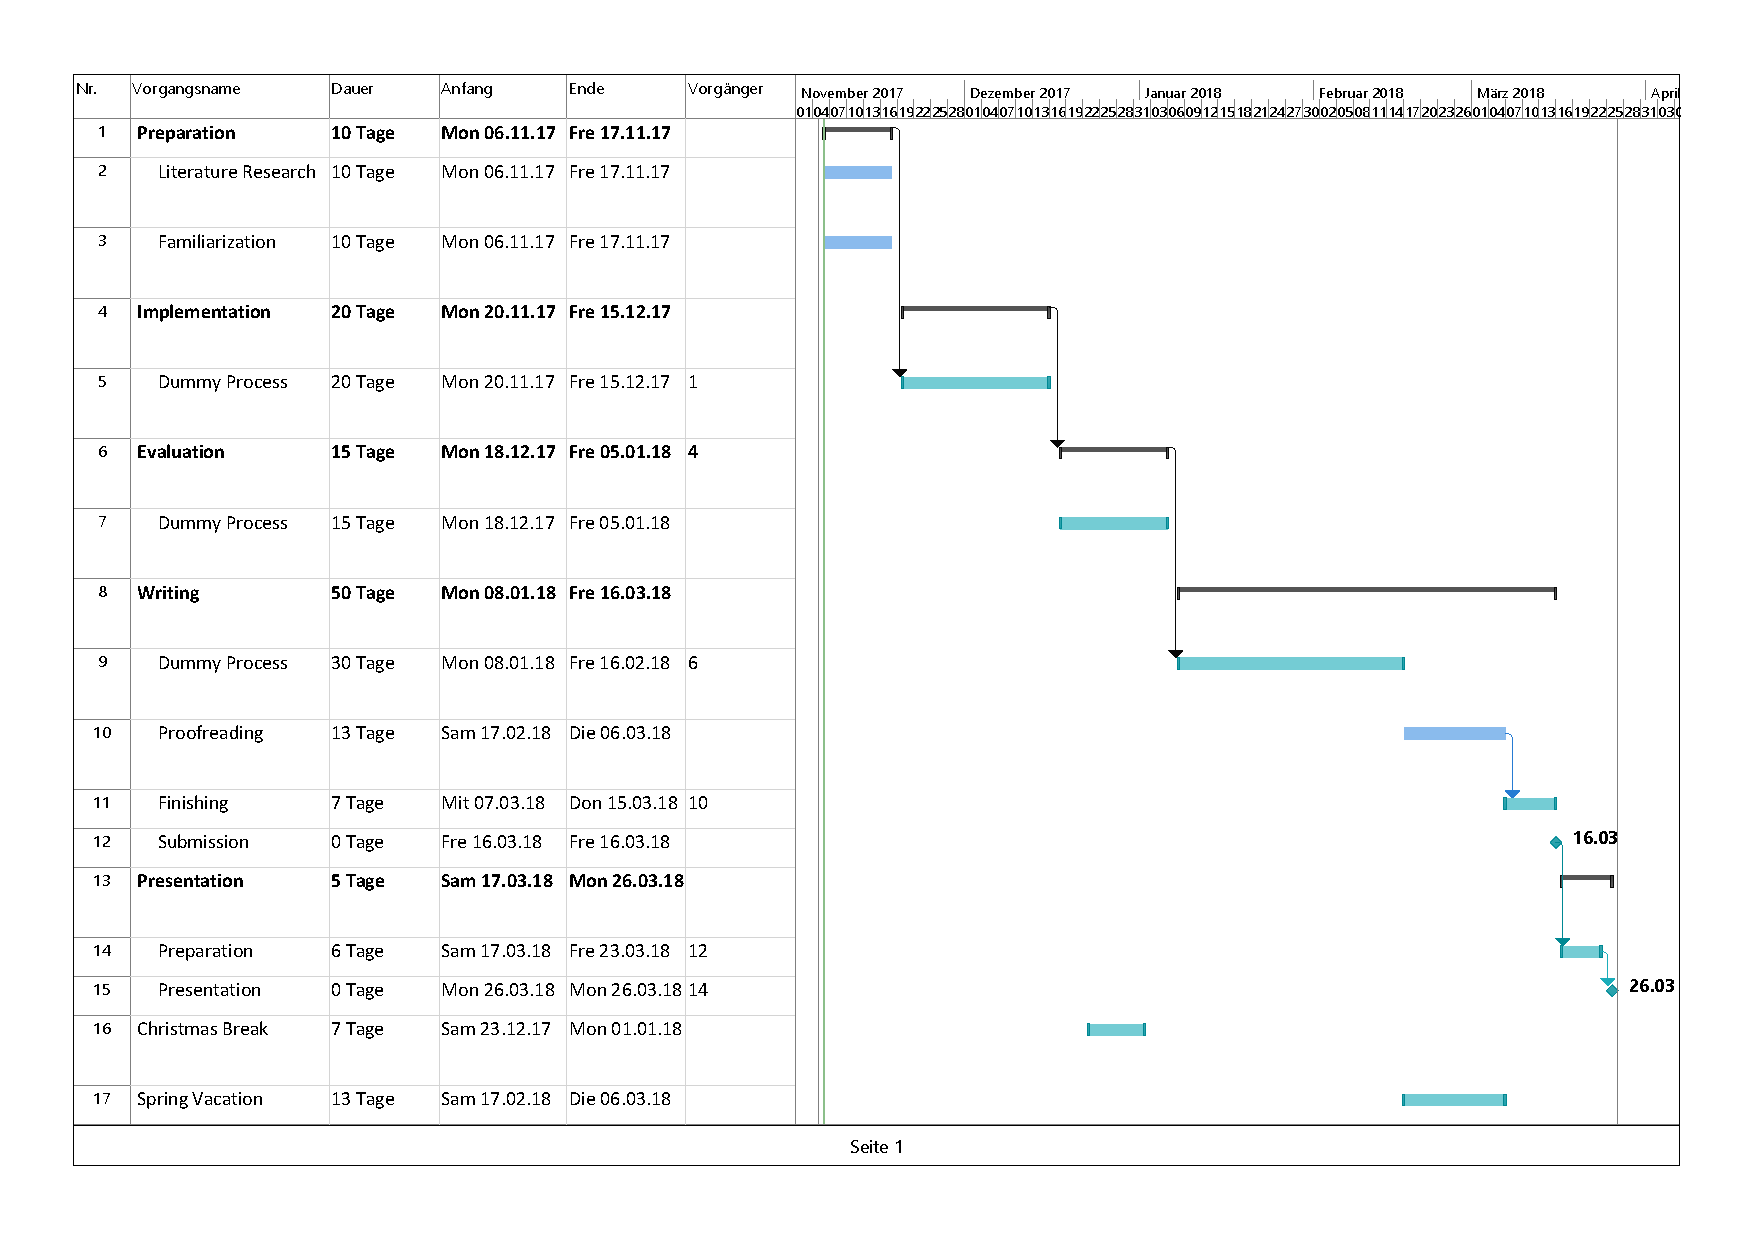
\includegraphics[angle=-90,width=.8\textwidth]{Gantt_BA_Helena}
	\caption{Sketch of the time schedule for the work on the thesis}
	\label{fig:time-schedule}
\end{figure}
% % %

\newpage

\bibliography{literature}
\bibliographystyle{myalphadin}

\vspace{6cm}

\begin{center}
     \begin{tabular}{l p{0.1\textwidth} r}
       \cline{1-1} \cline{3-3}
       \begin{minipage}[t]{0.4\textwidth}
         \centering
         Supervisor\\(Prof. Dr. Eyke H\"ullermeier)
         \end{minipage}
&
         \begin{minipage}[t]{0.2\textwidth}
         \end{minipage}
&
         \begin{minipage}[t]{0.4\textwidth}
           \centering
           Student\\(Helena Graf)
         \end{minipage}
     \end{tabular}
\end{center}

\end{document}
